\chapter{Subsystems}
\label{chap:subsystems}
.....



\section{Rover}
\label{sec:rover}
...
\section{Structure and Mechanics}
\label{sec:mechanics}
...
\section{Communications and Command and Data-Handling}
\label{sec:comm}
...
\section{Payload}
\label{sec:payload}
...
\clearpage
%-------------------------------------------------------------------------------
\section{Thermal Control System} \label{sec:thermalcontrol}
%-------------------------------------------------------------------------------
The main object of the Thermal Control System (TSC) is to keep the eletric components within their temperature limits, listed in \autoref{tab:tcs_limits}.
As a result of Europas low ground temperature, a small solar constant and the thin atmosphere the heat loss of the rover has to bin minimised.
This shall be reached by a smart heat distribution as well as by an adequate insulation and surface finishing.
\\
The main heat source of the rover is the waste heat of the RTG (see \autoref{sec:EPS}), which will be lead by thermal straps to the thermal critical components.
The camera, exposed on a mast, will be heated by a seperat Radioisotope Heater Unit (RHU), cite{RHU}. % https://rps.nasa.gov/power-and-thermal-systems/thermal-systems/light-weight-radioisotope-heater-unit/
For the insulation, the material \textit{aerogel} will be applied, which has a very low heat conductivity (cite aerogel) and has also been used in space applications (cite{aerogel}).
The overheating of the rover shall be prevented by heat switches (see \autoref{fig:tcs_switch01}).
These components change their heat conductivity beyond a certain temperatur due to the expansion of the disk (see \autoref{fig:tcs_switch02}).
It was assumed, that the toggle temperatur can be adapted by increasing the disk height.
The influence of the changed disk stiffens on the contact pressure and the heat conductivity was neglected for this study.
The measured heat conductivity characterisitc was divided in three linear sections (\autoref{fig:tcs_switch22}), to enable a simple modelling in the upcoming thermal calculation.

\begin{figure}[h]
	\centering
	\subfloat[Closed]{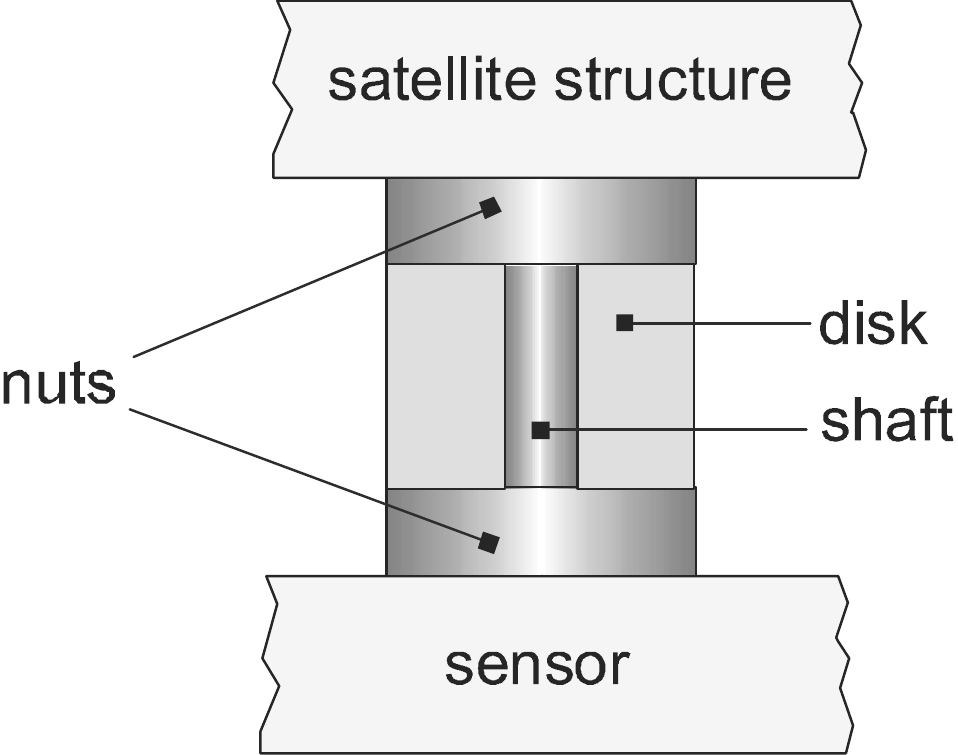
\includegraphics[height=0.17\textwidth]{Media/tcs_switch_01.png}\label{fig:tcs_switch11}}\qquad\qquad
	\subfloat[Open]{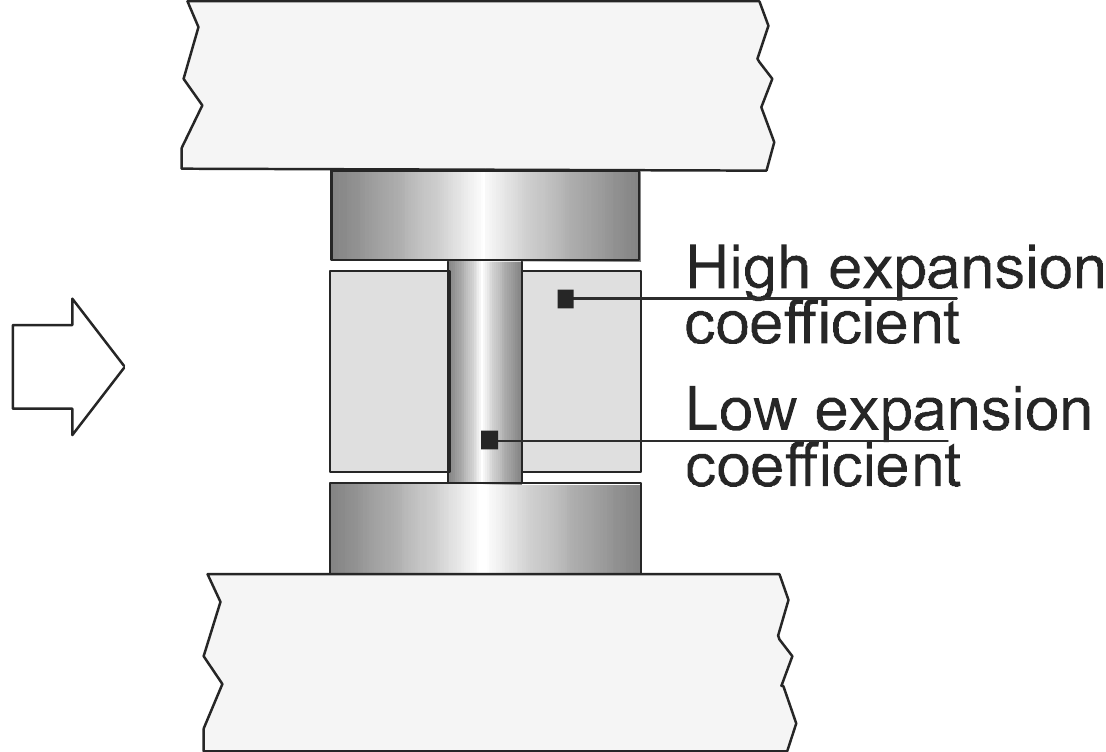
\includegraphics[height=0.17\textwidth]{Media/tcs_switch_02.png}\label{fig:tcs_switch12}}
	\caption{Heat switch.}
	\label{fig:tcs_switch01}
\end{figure}

\begin{figure}[h]
	\centering
	\subfloat[Original]{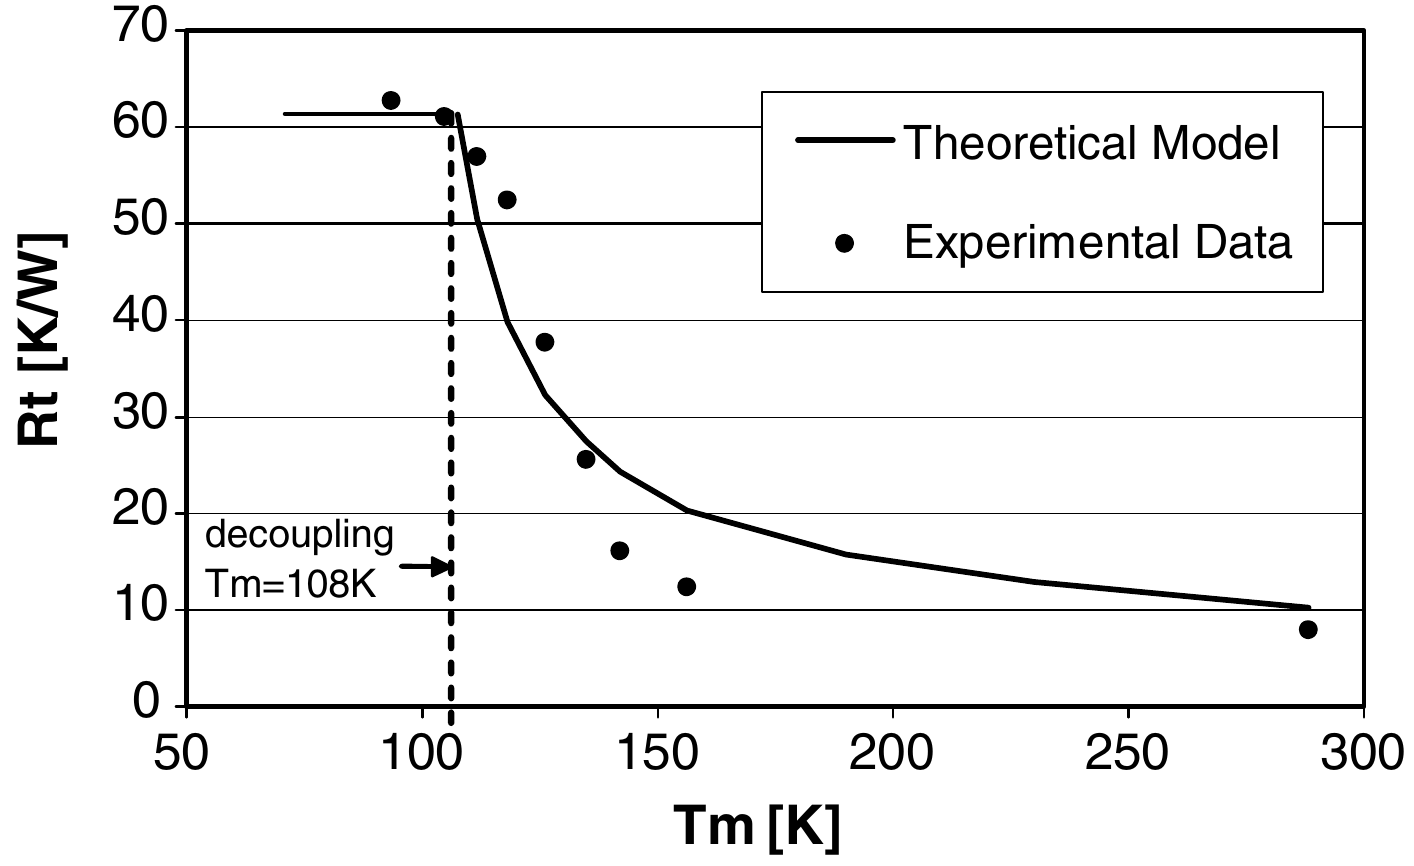
\includegraphics[height=0.25\textwidth]{Media/tcs_diag_orig.png}\label{fig:tcs_switch21}}\qquad
	\subfloat[Linearised]{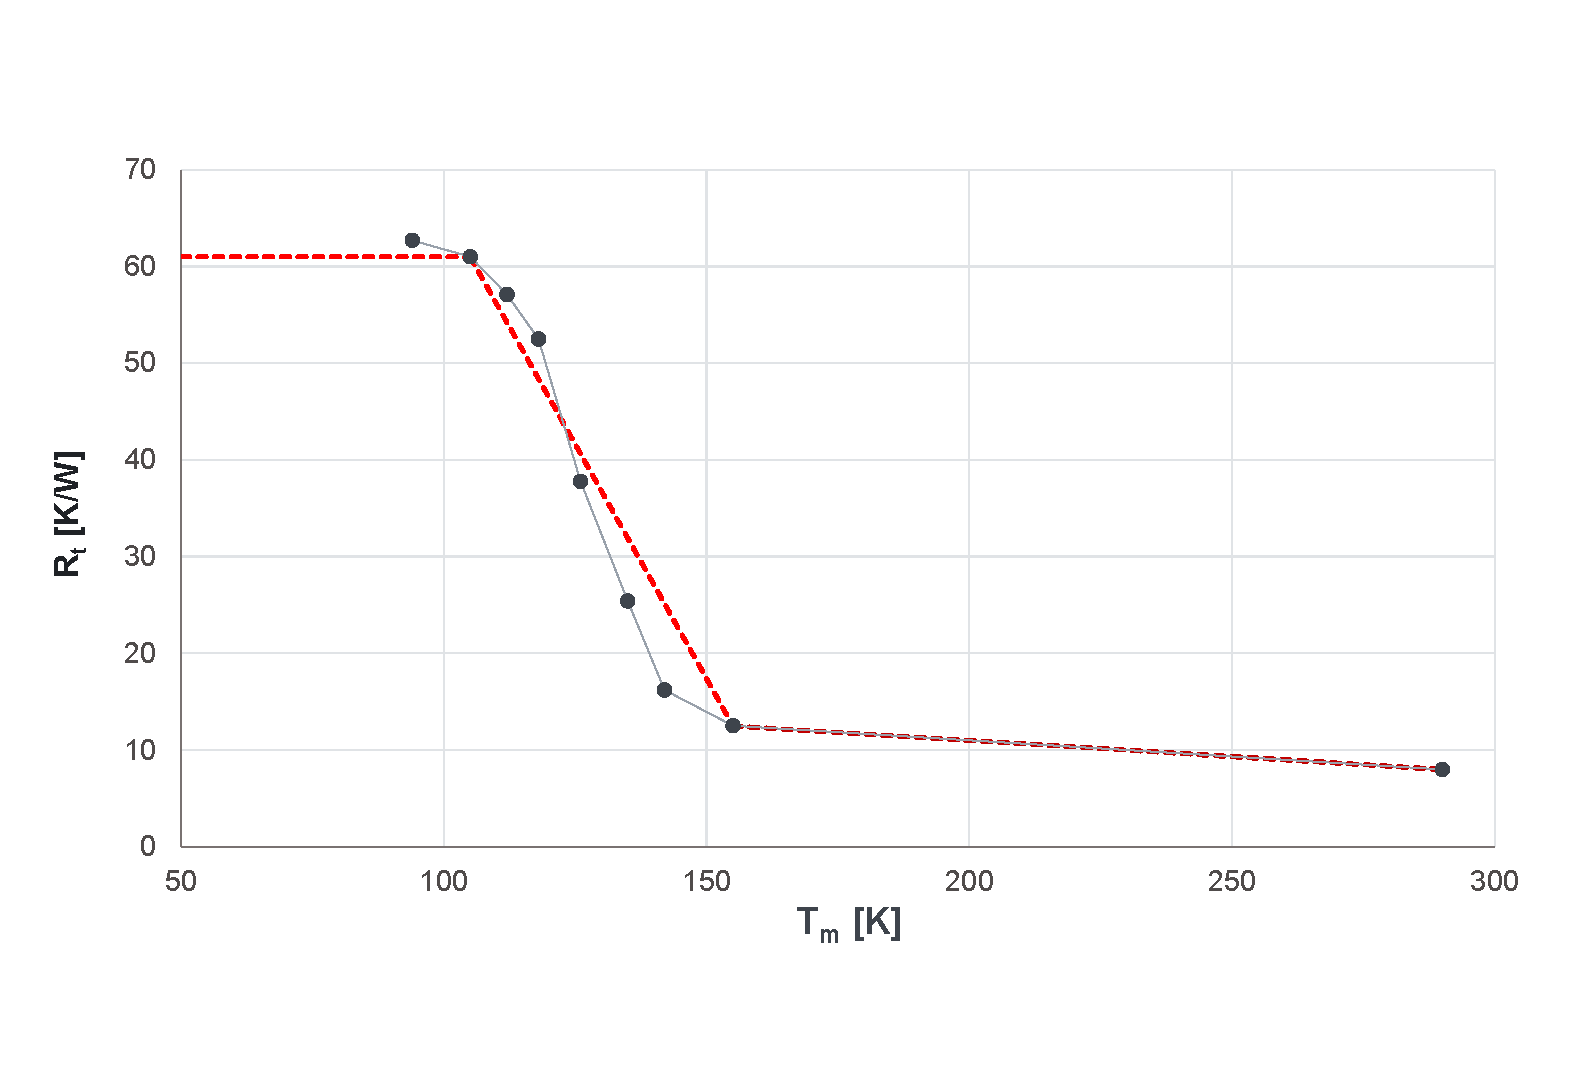
\includegraphics[height=0.25\textwidth]{Media/tcs_diag_lin}\label{fig:tcs_switch22}}
	\caption{Change of the heat switch conductivity $R_t$ over the mean temperature $T_M$.}
	\label{fig:tcs_switch02}
\end{figure}


A thermal analysis, which was performed to get
\begin{itemize}
	\item the dimension of the isnulation and heat straps,
	\item the necessary amount of RHUs and heat switches,
	\item the required surface finishing.
\end{itemize}



For that, a thermal network with ten nodes was derived from the rover, shown in \autoref{fig:tcs_network}.
At the intersection of the steering and drive engien, two additional nodes were defined to calculate the heat flow.


\begin{figure}[H]
	\centering
	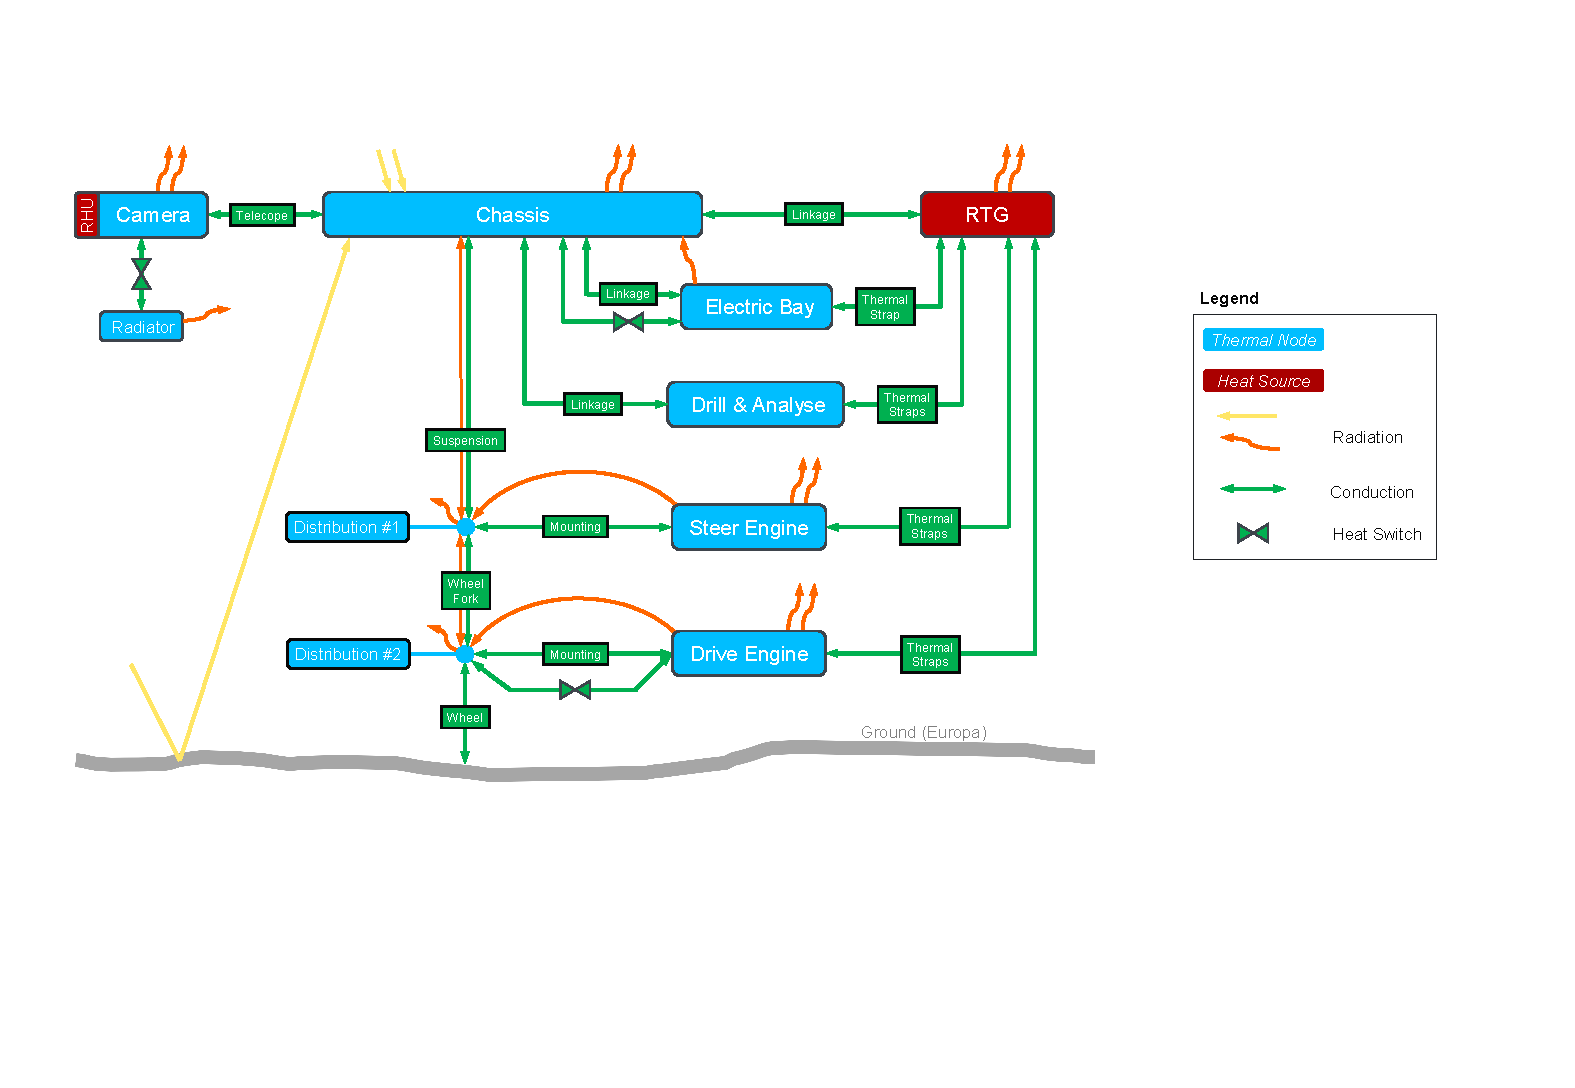
\includegraphics[width=1\textwidth]{Media/tcs_network}
	\caption{Thermal network of the rover.}
	\label{fig:tcs_network}
\end{figure}

On the basis of the thermal network, the heat energy equlibrium for each node was defined (see \autoref{sec:AppendixThermal}).
The calculation were considered as a quasi-static analysis, were the component temperatures stay constant, $\frac{\text{d}T}{\text{d}t}=0$.
Due to the early state of the rover, simplifications and asumptions were made.
\begin{itemize}
	\item The convection was neglected due to the thin atmosphere.
	\item The whole electrical power of the components will be dissipated into heat.
	\item A variation of $\pm 20\%$ for the emisivity and absorpsivity values were considered, if applicable (seet \autoref{tab:tcs_surface}).
	\item The heat as a result of retardation radiation inside the shielding was neglected.
	\item The E-Bay emitts heat energy only in one direction to the chassis.
	\item Only the chassis and the camera absorb sun radiation, detailed description see \autoref{sec:app_therm_4}.
	\item The ice core drill and the APXS analyser were summerised as one single node.
	\item There aren't dicrete nodes for the radar, hazcams and deployment engines. Their heat will be lead into the chassis.
	\item The thermal resistance between two surfaces was neglected because of the lack of necessary values. Therfore, the heat conductivity was reduced about $10\%$.
	\item There is no heat loss of the thermal straps. This can be compensated by increasing the cross section.
\end{itemize}




There were different load cases defined not only to cover the most important hot and cold cases but also some relevant operating cases.



The thermal analysis was perfomred as a Excel calculation, which can be found in the corresponding folder of Team 3.



The results of the temperatures for each node at each for the hot and cold cases  are listed in autoref{tab:}.
The temperature margins for uncertainties, acceptance tests and qulification tests were considered with $5 K$ each, $\pm 15K$ in total.
The corresponding temperatures are listed in autoref{tab:}.
All temperature lay betwenn their limits.

\begin{table}[htb]
	\centering
	\begin{tabular}{l@{\qquad\qquad}cc@{\qquad}|@{\qquad}cc}
		\hline
		Components & \multicolumn{4}{c}{Load Case}   \\ \hline
		 & \multicolumn{2}{l}{Hot case} & \multicolumn{2}{l}{Cold case} \\
		  & $0K$ & $+15 K$ & $0K$ & $-15 K$ \\ \hline
		RTG  & 380 & 395 & 350 & 335   \\
		Electric Bay & 310 & 325 & 261 & 246  \\
		Drill \& Analyser & & & &  \\
		Camera & & & &  \\
		Steering Engine & & & &  \\
		Drive Engine & & & &  \\   \hline
	\end{tabular}
	\caption{Temperature results in $K$ of thermal analysis.}
	\label{tab:tcs_temp}
\end{table}

In a furher step, a more detailed analysis has to be carried out with the Finite-Element-Method to identify the correct heat and temperature distribution.\\

\clearpage
%-------------------------------------------------------------------------------
\section{Electrical Power System}
%-------------------------------------------------------------------------------
\label{sec:EPS}
The EPS (Electrical Power System) is the subsystem responsible for the electrical power supply of INSPIRE. It consists of four funadmental parts, which are the energy source, the PCDU unit (Power Control and Distribution)and the Energy Storage as well as the rover subsystems as the consumers. The EPS is visualized in \autoref{fig:epsflowchart}.

\begin{figure}[htb]
{\centering
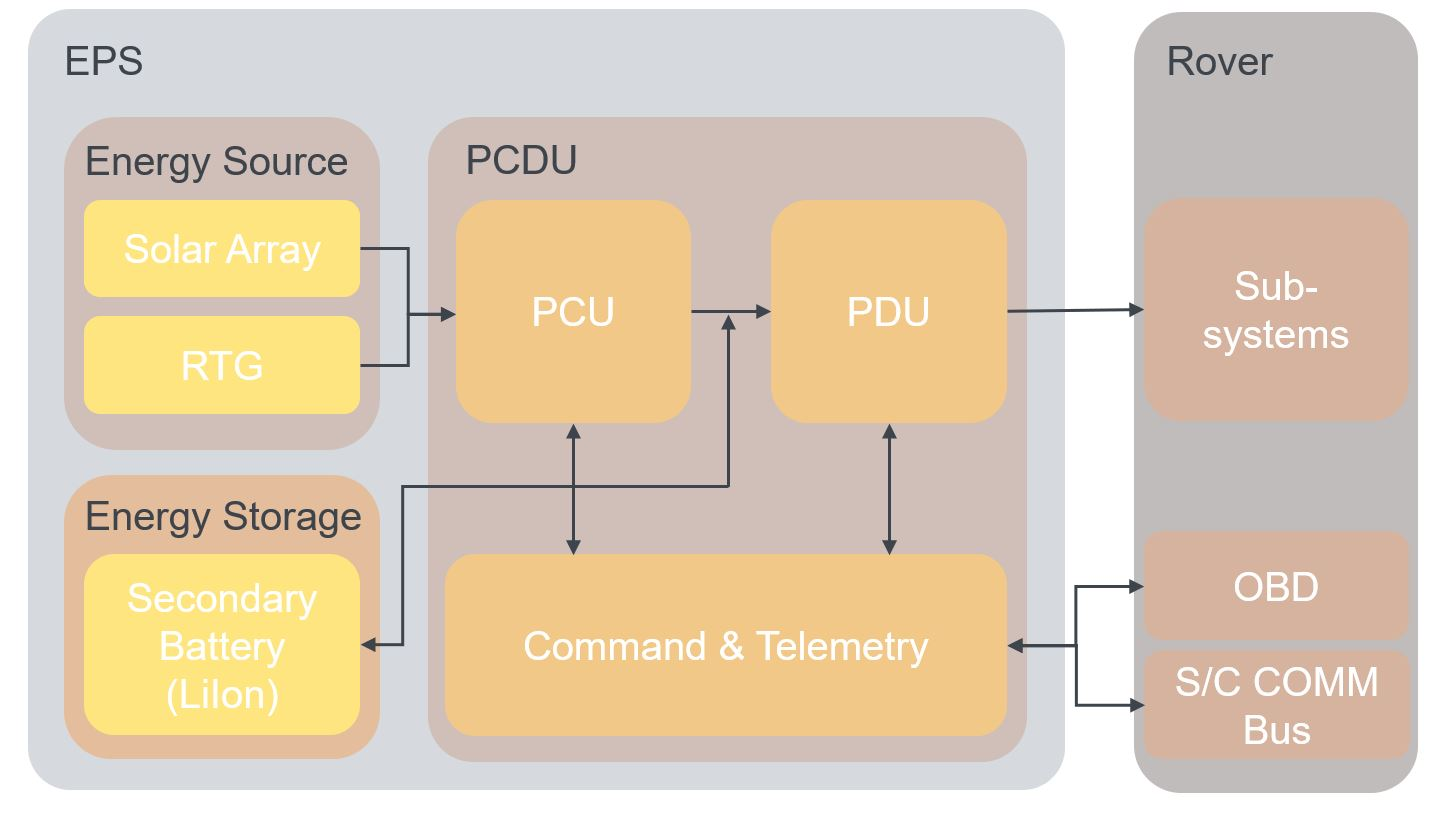
\includegraphics[width=0.7\textwidth]{Media/epsflowchart}
\caption{Functional Flow Chart Diagram for the EPS Subsystem.}
\label{fig:epsflowchart}
}
\end{figure}


\subsection{EPS Budget and Overview}
\autoref{tab:powbud} summarizes the power budget of INSPIRE based on the rover system modes defined in \autoref{chap:rovsubmod}. The complete power budget can be found in \autoref{tab:powerbudgetcomplete}.
As can be seen, the Locomotion mode has the highest demands on the EPS. Communication mode also has a high consumption. However, since this is primarily used at night and the rover can be charged again afterwards without any problems, it does not place any major restrictions on the power budget. Idle/Perception mode has a low consumption, but is usually used for a long time at a stretch and therefore also places high demands on the EPS. In Charging mode, the EPS is able to charge $7.04 \ W_{el} $.


\begin{table}[htb]
\centering
\begin{tabular}{|c|c|}
\hline
\textbf{Rover System Mode} & \textbf{\begin{tabular}[c]{@{}c@{}}Total Rover \\ Power Demand \\ including battery charge $P_\text{mode}$ [$W_{el}$]\end{tabular}} \\ \hline
Idle/Perception            & $15.25$                                                                                                                             \\ \hline
Safe/Hibernation           & $-5.84$                                                                                                                             \\ \hline
Communication              & $36.92$                                                                                                                             \\ \hline
Charging                   & $-7.04$                                                                                                                             \\ \hline
Locomotion                 & $232.36$                                                                                                                            \\ \hline
Payload: Observation       & $15.41$                                                                                                                             \\ \hline
Payload: Ice Core Mode     & $9.77$                                                                                                                              \\ \hline
\end{tabular}
\caption{Overview of the Power Budget of INSPIRE.}
\label{tab:powbud}
\end{table}


\subsection{Energy Source}
For the energy generation of INSPIRE many possible sources were taken into consideration for a trade-off. As a conclusion of this trad-off the decision was made to utilize a Radioisotope Thermoelectric Generator (RTG) as the main energy source for INSPIRE.\\
As the research couldn't find an RTG with a mass suitable for INSPIRE, the solution was to scale down a bigger RTG as an approximation. As a baseline of the scaling the eMMRTG (Enhanced Multi Mission Radioisotope Thermoelectric Generator) was utilized, which is currently under development at NASA and is especially designed for deep space missions like Europa. For the scaling a goal RTG mass of $m_\text{RTG}=3 \ \text{kg}$ was defined and the eMMRTG was scaled down using the given data.\\
In \autoref{tab:esmmrtg} the scaling results for the eSMMRTG (Enhanced and Scaled Multi Mission Radioisotope Thermoelectric Generator) are listed. The eSMMRTG has a BOL specific power of $\alpha_\text{BOL}= 4.0 \ \frac{W_{el}}{kg}$ and provides an electrical power of $P_{el} = 12.08 \ W_{el}$ during the mission duration\cite{R.Abelsonetal..2004}\cite{S.Magdum.2019}\cite{Holgate.2015}\cite{eMMRTG.NASA}\cite{Lakdawalla.2018}.



%The outcome of this trade-off is shown in \autoref{fig:epssourcetradeoff} for the most promising energy sources. 

%
%\begin{figure}[htb]
%{\centering
%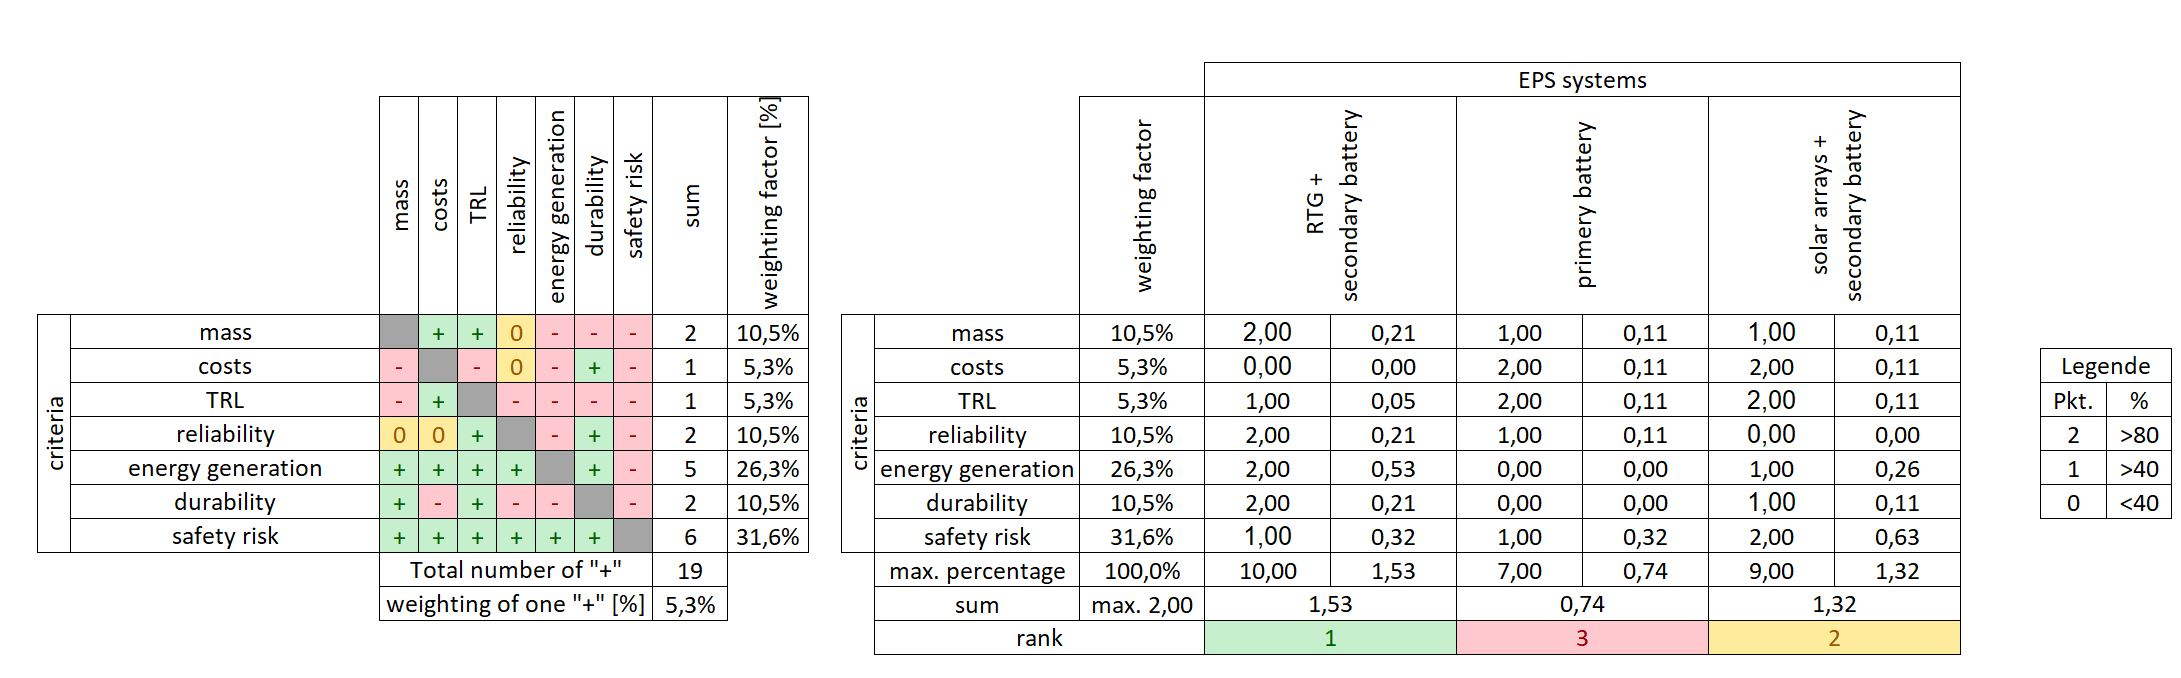
\includegraphics[width=0.7\textwidth]{Media/epssourcetradeoff}
%\caption{Trade-Off Conclusion for the EPS Energy Source.}
%\label{fig:epssourcetradeoff}
%}
%\end{figure}

\begin{table}[H]
\centering
\begin{tabular}{|c|c|}
\hline
\multicolumn{2}{|c|}{Scaled eSMMRTG Parameter}                \\ \hline
\textbf{System Mass} $m_\text{RTG}$ [$kg$]                             & \textbf{3.5}     \\ \hline
BOL Specific Power $\alpha_\text{BOL}$ $\frac{W_{el}}{kg}$  & $4.0$     \\ \hline
BOL Power $P_{el,\text{BOL}}$ $\ W_{el}$                    & $14$       \\ \hline
Isotrop                                                     & Pu-238   \\ \hline
Isotrop Half-Life [$a$]                                       & $87.7$     \\ \hline
Flight time and Storage (incl. Margins) [$a$]                 & $7$        \\ \hline
Power Loss Degradation until BOM $\ W_{el}$                 & $0.56$     \\ \hline
BOM Power $P_{el,\text{BOM}}$ $\ W_{el}$                    & $13.44$    \\ \hline
Europa Day Duration [$h$]                                     & $85$       \\ \hline
Mission Duration [$d$]                                        & $106.25$   \\ \hline
End of Mission Power $P_{el,\text{EOM}}$ [$\ W_{el}$]         & $13.42$   \\ \hline
\textbf{Final Power for Study} $P_{el}$ [$\ W_{el}$] (incl. $10\%$ scaling Margin) & \textbf{12.08}    \\ \hline

\end{tabular}
\caption{Parameters for the scaled eSMMRTG based on the eMMRTG.}
\label{tab:esmmrtg}
\end{table}

Furthermore INSPIRE will also be equipped with some radiation hardend solar arrays as already explained in \autoref{subsec:radhard}\cite{FraunhoferInstituteforSolarEnergySystemsISE.2021}. Since these solar cells are primarily used for technology testing, the mission must also be able to operate completely without this generated energy. For this reason, and because the expected energy generated by the solar cells is minimal, only the energy generated by the RTG is considered for the Phase 0 Study. However, it should be noted that these solar cells will also generate a certain amount of energy, which will benefitial for the EPS.


\subsection{Energy Storage} 
For the energy storage of INSPIRE many possible battery types were taken into consideration for a trade-off. As a conclusion of this trad-off the decision was made to utilize LiIon batteries as the secondary batteries of INSPIRE. This decision is primarly based on LiIon batteries high energy density, temperature range, robust performance and long operating and cycle life in extreme environments\cite{IRSatUniversityofStuttgart.2020}. \\
As the RTG only generates a small constant power the main energy source during the mission will be the accumulated energy of the batteries. The rover will charge the batteries at night, so the next exploration day can start with full capacity. Furthermore the batteries have to be charged during day time to maintain operations.\\
For the sizing of the batteries, the rover motion was chosen as the design driver, since this is the highest energy consuming state of the rover and additionally mission critical for INSPIRE. The rover motion consists of an interaction of the Locomotion and Perception mode as already mentioned in \autoref{chap:Operation}. Therefore it was defined that INSPIRE shall be able to drive $ 50 \ m $ (including alternating Locomotion and Perception Mode) with a fully charged Battery. The required battery capacity $C_\text{Batt,req}$ can be caculated using \autoref{eq:batreq}. The results are listed in \autoref{tab:batsize} \cite{S.Klinkner.2021}.


\begin{equation}
C_\text{Batt,req} = \frac{P_\text{el,req} \cdot t_e }{DoD \cdot \eta_\text{LiIon}}
\label{eq:batreq}
\end{equation}

\begin{table}[htb]
\centering

\begin{tabular}{|l|c|c|}
\hline
\textbf{Power Consumption Mode:}                        & \textbf{Locomotion} & \textbf{Perception} \\ \hline
Required Electrical Power $P_\text{el,req}$ [$W_{el}$]         & 283.43              & 14.01               \\ \hline
Duration of the mode $t_e$ [$s$]                          & 500              & 15000            \\ \hline
$DOD$ for Dimensioning [-]                              & 0.90                & 0.90                \\ \hline
Efficiency of LiIon Cells $\eta_\text{LiIon}$ [-]       & 0.95                & 0.95                \\ \hline
Required Battery Capacity per mode $C_\text{mode}$ [$Wh$] & 46.04               & 68.27               \\ \hline
\textbf{Total Required Battery Capacity} $C_\text{Batt,req}$ [$Wh$]    & \multicolumn{2}{c|}{\textbf{114.32}}               \\ \hline
\end{tabular}

\caption{Power consumption mode used as design case for the battery sizing.}
\label{tab:batsize}
\end{table}

Using these values a suitable battery cell and battery design configuration were conducted. Under consideration of these parameters the battery capacity $C_\text{Batt}$ can be calcuated:

\begin{equation}
C_\text{Batt} = C_\text{cell} \cdot V_\text{cell} \cdot N \cdot M .
\label{eq:batuse}
\end{equation}

According to the ECSS reliability restrictions 1 battery string must be substracted for dimensionsing. Furthermore a $30 \%$ margin on the energy content was applied. This leads to a final battery configuration with a capacity of $C_\text{Batt}=138,88 \ Wh$ and a mass of $m_\text{Batt} = 1980 \ g$. The final battery values are listed in \autoref{tab:battery} \cite{SAFTBatteries.2018}.


\subsection{EPS Power Control and Distribution}
In order to ensure the full functionality of the EPS, the last main component to be selected is a suitable PCDU. As described in \autoref{fig:epsflowchart}, the PCDU forms the heart of the EPS and is an important interface to the OBC and COMM. Furthermore the PCDU shall be able to monitor and control the rover system if necessary through watchdogs, HPC (High Priority Commands) and direct connections to the OBC and COMM.\\
The PCDU has the challenging task not only to process the RTG as the main energy source, but also to process solar cells as secondary energy sources. Therefore, a PCDU was sought which has the required size, dimensions and range of functions. The research resulted in the Nova PCDU from Bradford DSI. In addition, margins were added to the PCDU to ensure feasibility\cite{BradfordSpace.2019}.

\clearpage
%-------------------------------------------------------------------------------
\section{Radiation} \label{sec:Radiation}
%-------------------------------------------------------------------------------

Compared to the radiation environment near Earth the radiation environment near Jupiter is multiple times stronger. It has the highest radiation levels of any planet in our solar systems \cite{Platzhalter}. In order to survive these harsh environmental conditions, special emphasis must be placed on the radiation protection. In \autoref{fig:trappedprotonelectronfluxes}, the average trapped proton and electron fluxes on Europa's orbit around Jupiter are shown in comparison to the outer Van Allen radiation belt around Earth. However, in contrast to the Van Allen radiation belt, the duration within the radiation environment on Europa cannot be minimised and the rover has to be designed to withstand the entire mission duration of 30 days. \\ \\
In oder to design and evaluate different radiation protection approaches, different calculations have to be performed. For this purpose the ESA SPace ENVironment Information System (SPENVIS) is used \cite{Platzhalter}. All calculations and figures in \autoref{sec:Radiation} are performed with SPENVIS unless otherwise stated.

\subsection{Radiation Protection}

Various options are available to protect the rover against the radiation. A common approach is the use of aluminium or titanium as these materials can also act as structural elements. However, due to the mass constraints of 30 kg other materials or material compositions are taken in consideration which are more mass effective. In \autoref{tab:OptimalRadiationProtection}, an optimised shield structure is presented for different weight thresholds designed for the radiation environment around Jupiter.

\begin{wraptable}{r}{8cm}
\centering
\caption{Optimal shield structure for an Jupiter mission. \cite{Platzhalter}}
\begin{adjustbox}{max width=\textwidth}
\begin{tabular}[l]{cccccc}

	\toprule
	
	Areal Density	&	\(0.5\)	&	\(1\) &  \(2\) & \(3\)	\\
	/ \(\text{g/cm}^2\)	&	&	&  & \\
	
	\midrule
	
	
	Layer No. 1	&	Pb &  Pb & W	& Ta	\\
	/ mm	&	0.415 &  0.829 & 0.984	& 1.563	\\
	
	
	Layer No. 2	&	Fe	&  Mg &	Mg & Al \\
	/ mm	&	\(0.033\)	&  \(0.158\) &	\(0.540\) & \(0.399\) \\
	
	
	Layer No. 3 &	-	&  -	& - & Mg \\
	/ mm &	-	&  -	& - & \(0.150\) \\
	

	\bottomrule

\end{tabular}
\end{adjustbox}
\label{tab:OptimalRadiationProtection}
\end{wraptable}

The difference between an aluminium or titanium shielding and an optimised structure listed in \autoref{tab:OptimalRadiationProtection} for the total ionizing dose (TID) is shown in \autoref{fig:AluminiumTitanOptimised}. \\ \\
Due to the mass savings of the optimised structure it will be used where the radiation protection of the aluminium structure is not sufficient. In order to reduce the mass further, a radiation vault is utilised that highly sensible components do not have to be shielded separately.

\subsection{Components}

Every component on the rover has a different radiation tolerance and therefore have to be placed at different compartments within the rover. The radiation tolerances are listed in \autoref{tab:RadiationList}. None sensitive components like the electric motors and harness are only shielded by an aluminium structure where components like the metal within the wire are resistant against the radiation. However, isolators around the cables have to be selected to be resistant in order to prevent short circuits. Highly sensitive components like cameras have an additional protective layer in order to reduce the TID to under 30 krad. Components which are within the rover like the on-board computer (OBC) are placed within the radiation vault which reduces the TID to under 20 krad. For this purpose the optimised shield structure with a weight target of 0.5 \(\text{g/cm}^2\) is used. Detailed TIDs for all components are shown in \autoref{fig:CompartmentTID}.

\subsection{Improvements}

Even though the radiation protection is sufficient for the rover to survive at least the nominal mission of 30 days, further improvements can be performed in order to extend the secondary mission. \\ \\
Local shielding can be applied on less resistant components in order to reduce the wall thickness of the whole radiation wall. If components with a radiation tolerance under 30 krad are individually shielded a mass saving of xx \% can be achieved. Additionally, water ice extracted from the surface of Europa can be used to improve the radiation protection. With a layer of one centimetre of water, the TID within the radiation vault can be reduced by xx \%. \\ \\
Detailed calculations for local shielding and water improvements can be found in \autoref{Platzhalter} and may be analysed further in Phase B.

\subsection{Conclusion}

In order to protect the rover against the high radiation levels at the surface of Europa, the rover has different compartments. High sensible components are placed within a radiation vault which has a mass optimised structure. Components which has to be outside the radiation vault but are highly sensible are shielded individually. Low sensible Components are protected by the Aluminium structure. \autoref{fig:RadiationOverview} illustrates the different compartments within the rover and the accorded TIDs.

\begin{figure}[htb]
     \centering
     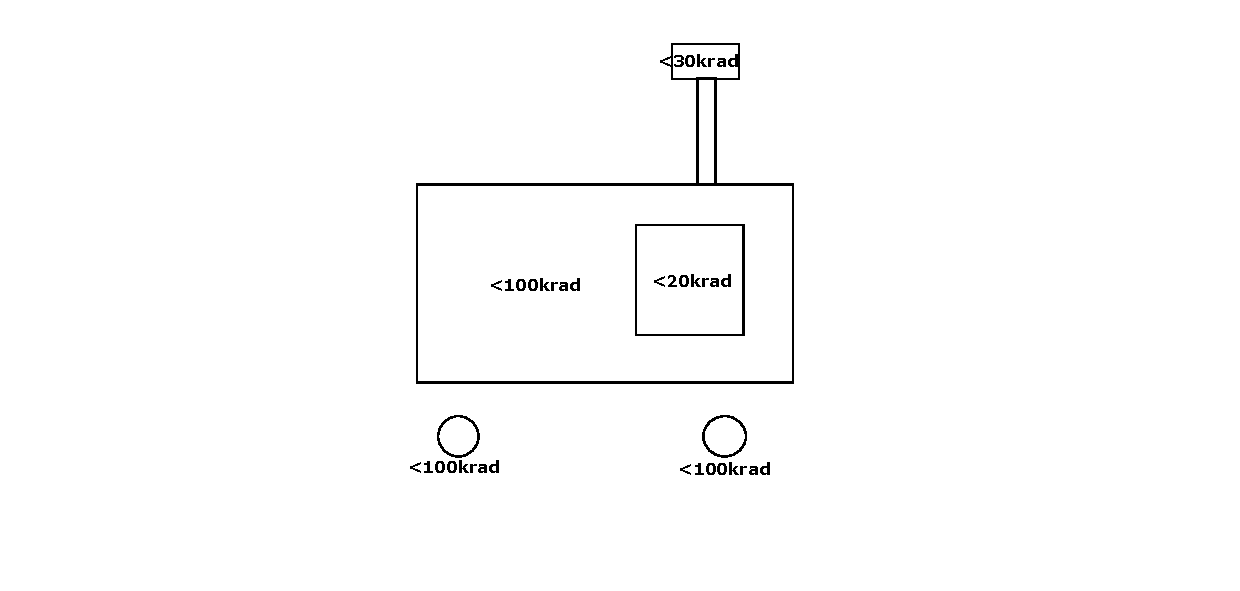
\includegraphics[width=\textwidth]{Media/RadiationOverview}
     \caption{Overview of TIDs within different compartments within the rover.}
     \label{fig:RadiationOverview}
\end{figure}

\clearpage

%-------------------------------------------------------------------------------
\section{Locomotion} \label{sec:locomotion}
%-------------------------------------------------------------------------------

\subsection{Deployment mechanism}

%-------------------------------------------------------------------------------
\section{Control and Autonomy} \label{sec:ControlandAutonomy}
%-------------------------------------------------------------------------------

\cleardoublepage